\chapter{تعریف مسئله و مفاهیم مقدماتی}
\section{مروری بر موسیقی}
بدون شک موسیقی یکی از غنی‌ترین و قدیمی‌ترین بخش‌های تمدن بشری هست. اولین ساز
حدود چهل و پنج هزار سال پیش ساخته شد و تا امروز این شکل هنر به رشد خود ادامه‌
داده است. در این بخش مروری کوتاه بر مفاهیم موسیقیایی استفاده شده در این
پایان‌نامه انجام شده است.

\subsection{نت موسیقی}
مهم‌ترین بخش پایه‌ای موسیقی نت هست که می‌توان آن را با سه مفهوم \gls{pitch}،
\gls{velocity} و \gls{timber} توصیف کرد. \gls{pitch} فرکانس پایه‌‌ی صوت تولید
شده توسط ساز هست. \gls{pitch} واضح‌ترین فرکانس قابل درک نت هست. \gls{pitch}
زیرتر به معنی فرکانس بالاتر هست. \gls{velocity}، قدرت نواختن نت را مشخص می‌کند.
نت‌های که \gls{velocity} بالاتری دارند قابل درک‌تر هستند. همچنین معمولا نت اول
هر کلمه موسیقیایی \gls{velocity} بالاتری دارد. درنهایت \gls{timber} اشاره به شکل
سیگنال صوت تولید شده دارد. دو نت می‌توانند \gls{pitch} یکسانی داشته باشند ولی
شکلی که این نوسان انجام می‌شود متفاوت باشد. این تفاوت را با \gls{timber} ساز
بیان می‌کنند. \gls{timber} مفهومی هست که باعث تفاوت صدای سازهای مختلف می‌شود. در
شکل۱.۱ نمونه‌ای از \gls{timber} ساز ویولن نشان داده شده است.
\begin{figure}
    \centering
    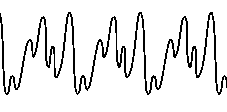
\includegraphics[height=2.5cm]{./statics/note_visualized.png}
    \caption{نمونه‌ای از \gls{timber} ویولن}
\end{figure}

همچنین هر نت یک زمان شروع یا onset و یک زمان پایان یا offset دارد. هرچند در بعضی
از سازها این مرزها کاملا مشخص و قابل تفکیک نمی‌باشند. برای مثال در پیانو پس از
رها کردن یک کلاویه همچنان ساز می‌تواند صوتی تولید کند.

وقتی از نواختن چند نت به صورت همزمان صحبت می‌کنیم معمولا مجموعه‌ای از نت‌ها با
هم صدایی خوش‌آیندتر تولید می‌کنند. به این مجموعه‌ی نت یک \gls{chord} گفته
می‌شود. یک \gls{chord} معمولا شامل نت‌هایی می‌شود که هارمونیک مشابه و نزدیک به
هم دارند. نت‌هایی که فرکانس پایه‌های آن‌ها با هم نسبت ۴، ۵، ۶ دارند نمونه‌ای از
یک \gls{chord} معروف هستند. به عنوان نمونه‌ای دیگر از \glspl{chord} مشهور
می‌توان به دو نت با نسب فرکانسی ۱ و ۲ اشاره کرد.

\subsection{پیانو}
پیانو یک ساز از خانواده ساز‌های صفحه‌کلیددار است که در سال ۱۶۹۸ اختراع شد. این
ساز در حالت استاندارد شامل ۸۸ کلید یا به اصلاح کلاویه هست که هرکدام نماینده یک
نت هستند. یکی از خصوصیات جالب این ساز این هست که پس از این که نوازنده شروع به
نواختن یک نت کرد تنها کنترلی که بر روی آن می‌تواند اعمال کنند یا رها کردن کلاویه
هست که باعث افت در شدت صدا می‌شود و یا دوباره نواخت همان نت هست.

همچنین این ساز شامل چندین پدال هست. مهمترین این پدال‌ها، پدال \gls{sustain} هست
که در صورتی که توسط نوازنده فشرده شده باشد، حتی رها کردن کلاویه باعث می‌شود صدای
آن نت باقی بماند. درنتیجه حتی اگه کلاویه متناظر یک نت هم فشرده نباشد باز آن نت
فعال می‌ماند.

\subsection{نمایش موسیقی}
همانند زبان طبیعی، برای موسیقی هم راه حلی نیاز هست که بتوان آن را ذخیره و به
سایرین منتقل کرد. همچنین مانند زبان طبیعی، نمایش‌های مختلفی نیز برای موسیقی وجود
دارند که بعضی‌ از آن‌ها مختص یک ساز خاص هستند. در ادامه سعی می‌شود چندتا از
نمایش‌های استفاده شده در این پایان‌نامه بررسی شوند.

\subsubsection{موج صوت}
از دید فیزیک، موسیقی چیزی بجز تغییر در فشار هوا و نوسان ذرات ماده نیست. با کمک
پیشرفت تکنولوژی می‌تواند این نوسانات را طی اجرای یک قطعه موسیقی در طول زمان
اندازه گرفت و با ایجاد مجدد نوساناتی مشابه موسیقی را باز تولید کرد. این نمایش
بیشتر در بحث‌های پردازش سیگنال مورد توجه قرار می‌گیرد. برای استفاده از
\gls{sound wav} در کامپیوتر ابتدا نیاز هست تا این نمایش گسسته‌سازی شود.

\subsubsection{رابط دیجیتال سازهای موسیقیایی}
در یک فایل \gls{midi} شروع، پایان، شدت، نواک و بسیاری دیگر از اطلاعات مربوط به
یک نت را می‌توان ذخیره کرد. همچنین این نمایش راه‌کارهایی نیز برای تغییرات
پدال‌ها و سایر اطلاعات اضافه نیز دارا است. در نتیجه یک فایل \gls{MIDI} تمام
اطلاعات لازم برای باز اجرای کامل یک قطعه موسیقی را دارد. با این حال این
نمایش خوانایی کمی‌ دارد و ساختار کلی موسیقی را رعایت نمی‌کند. برای همین استفاده
از این نمایش محدود به ارتباط بین ابزارهای دیجیتال هست.

\subsubsection{رول پیانو}
\gls{pianoroll} نمایشی دیگری هست که به صورت تاریخی برای اجرای موسیقی به صورت
خودکار استفاده می‌شده است. این نمایش یک رول بزرگ هست که هر سطر این رول نماینده
یک بازه زمانی و هر ستون آن نماینده یک نت هست. خانه‌هایی که نت در آن‌ها فعال بود
سوراخ می‌شد تا ماشین بتواند آن را اجرا کند. با پیشرفت تکنولوژی این نمایش هم
پیشرفت کرد و بسیاری از نرم‌افزارهای مدرن از آن برای نمایش موسیقی استفاده
می‌کنند.

به صورت کلاسیک این نمایش راهی برای نگه‌داری \gls{velocity} هر نت ندارند. برای
همین امروزه این اطلاعات به صورت جداگانه نگه‌داری می‌شوند. همچنین اطلاعاتی مثل
پلادها نیز در این نمایش جایی ندارند.
\begin{figure}
    \centering
    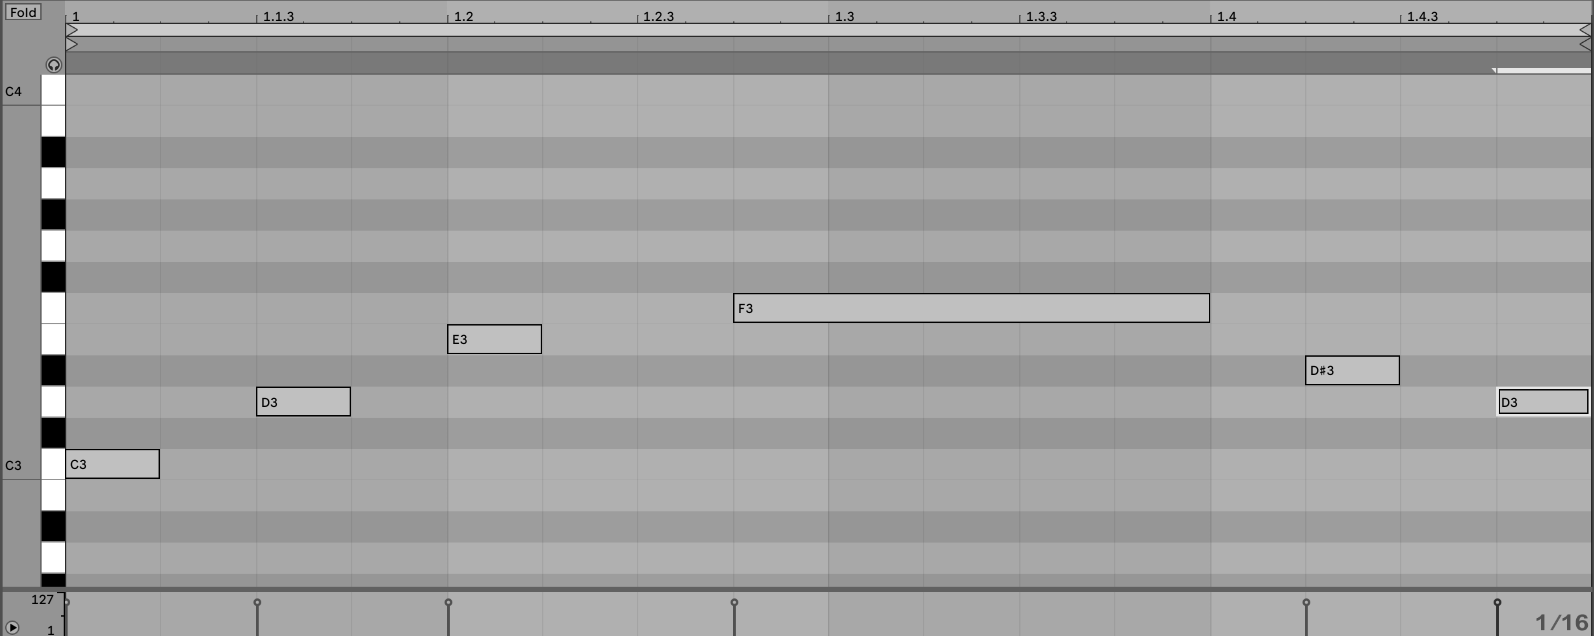
\includegraphics[width=12cm]{./statics/midi_piano_roll.png}
    \caption{نمونه‌ای از یک \gls{pianoroll} در یک نرم‌افزار کامپیوتری}
\end{figure}

\subsubsection{پارتیتور}
\gls{sheet music} نمایشی هست که در مدارس موسیقی آموزش داده می‌شود و عمدتا به
عنوان شکل نوشتار استاندارد موسیقی شناخته می‌شود. بررسی کامل این نمایش خارج از
دامنه‌ این پایان‌نامه هست و به صورت مستقیم در این پایان‌نامه استفاده نمی‌شود. به
صورت خلاصه در این شکل از نمایش مجموعه \glspl{pitch}‌ مجاز و \glspl{duration}‌
مجاز مشخص می‌شوند. سپس هر نت با توجه به مقدارهای تعریف شده بر روی خط‌های حامل
نمایش داده می‌شود.
\begin{figure}
    \centering
    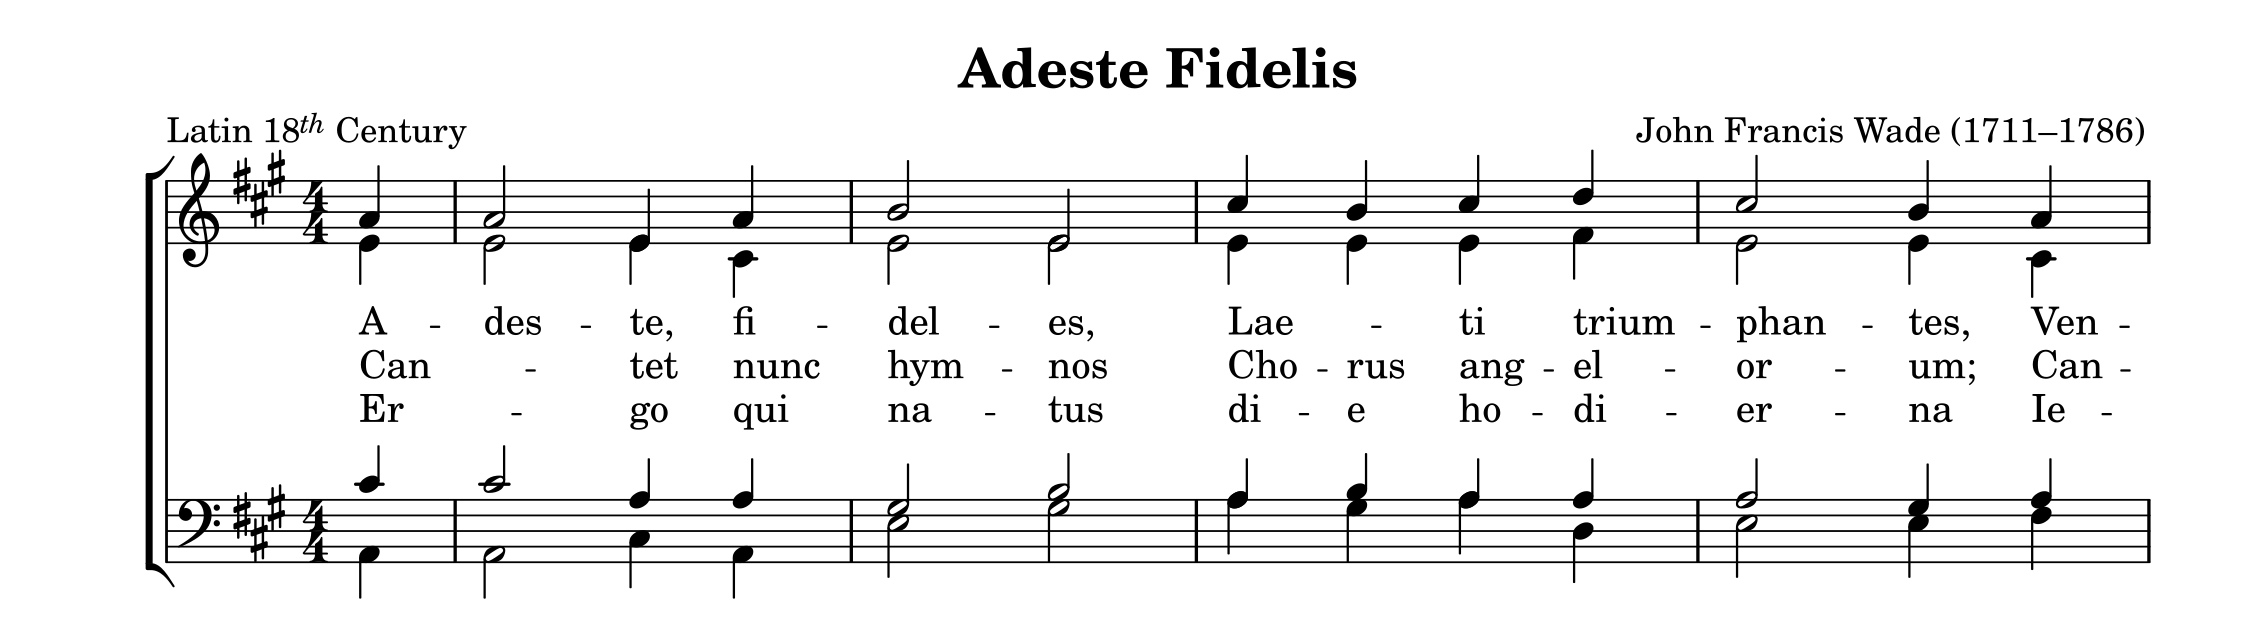
\includegraphics[width=12cm]{./statics/sheet_music.png}
    \caption{نمونه‌ای از یک \gls{sheet music}}
\end{figure}

\section{بازیابی اطلاعات موسیقیایی}
پیشرفت‌های تکنولوژی مانند شبکه، دیسک فشرده، ذخیره‌سازی ابری و موارد مشابه باعث
ایجاد حجم عظیمی داده در شکل‌های مختلف شده است. با توجه به این حجم از داده، نیاز
به سیستم‌هایی خودکار جهت استخراج اطلاعات از این داده‌ها کاملا مشهود است. یک
خانواده از روش‌های موجود برای طراحی این سیستم‌ها، روش‌های \gls{cbir} هستند. این
روش‌ها به ما امکان می‌دهند که بر روی داده‌های چندرسانه‌ای به جست‌وجو بپردازیم که
از ضعف‌های سیستم‌های جست‌وجوی فعلی است. در چند دهه اخیر \gls{CBIR} یکی از
موضوعات پرطرفدار جهت مطالعه بوده است و ابزارهای مختلف زیادی نیز در این حوزه
توسعه یافته است که برای مثال می‌توان به \gls{qbic} اشاره کرد. همچنین تکنولوژی
\gls{mir} کمک کرده است تا اطلاعات مورد نیاز از روی سیگنال‌های صوتی به دست آید.
به صورت کلی یک سیگنال صوتی، پدیده‌ای بسیار پیچیده است، زیرا شامل حجم زیادی
اطلاعات مرتبط با هنرمند، ژانر، احساس، ساز و غیره است. با توجه به تنوع بالا
اطلاعات موجود در این سیگنال‌ها، حیطه‌ی گسترده‌ای از مطالب در \gls{cbmir} جهت
مطالعه و بررسی موجود است.

برای \gls{cbmir} کاربردهای زیادی مانند مجموعه موسیقی شخصی‌سازی شده، توصیه
موسیقی، دسته‌بندی موسیقی، محافظت حق چاپ و غیره می‌توان متصور شد. برای توسعه این
کاربردها نیاز است که \gls{metadata} مورد نیاز از فایل‌های موسیقی استخراج شود ولی
از آن جا که متاسفانه این اطلاعات بر روی حجم زیادی از فایل‌های موسیقی قرار داده
نشده‌اند تنها راه موجود استخراج آن‌ها از روی سیگنال‌های صوتی است. همچنین انتظار
می‌رود \gls{CBMIR} برای مسائل زیر راهکاری داشته باشد:
\begin{itemize}
    \item تشخیص نواحی وکال در یک قطعه
    \item تشخیص هنرمند، سبک و نوع یک قطعه
    \item دسته بندی قطعات به دسته‌هایی مانند راک، جز، فولک، کلاسیک و غیره
    \item نوشتن خودکار متن یک آهنگ
    \item دسته بندی بخش‌های یک قطعه بر اساس بار احساسی آن بخش
    \item تشخیص نوع سازهای استفاده‌شده در یک قطعه مانند زهی، کوبه‌ای و غیره
    \item پیدا کردن قطعه‌های مرتبط به یک جستار به کمک معیارهای شباهت	
\end{itemize}

در ادامه به صورت خلاصه به معرفی بعضی از مهمترین مسائل این حوزه می‌پردازیم:

\subsection{قطعه‌بندی آواز و غیر آواز}
یک سیگنال صوتی از بخش‌های آواز، سازی، سکوت و یا ترکیب آواز و سازی تشکیل شده است.
تشخیص ساختاری یکی از مسائل جالب در این حوزه است. تشخیص نواحی سکوت یکی از اولین
قدم‌ها در هر سیستم پردازش گفتار و تشخیص صوت است. به صورت کلی طول بخش سکوت در هر
قطعه قابل چشم پوشی است زیرا بیش از ۹۹ درصد یک قطعه با صدای خواننده یا صدای ساز
پر شده است. بخش مشکل مسئله تشخیص آواز از صدای ساز است که در یک سیگنال موسیقی در
هم تنیده شده‌اند و بخش آوازی معمولا با یک موسیقی پس زمینه همراهی می‌شود. این
قسمت بندی پیش نیاز حل مسائلی دیگری مانند تشخیص خواننده، تشخیص بار احساسی، تشخیص
ساز و رونویسی متن آواز است.

\subsection{تشخیص هنرمند}
هنرمند یکی از مهم‌ترین اجزای هر قطعه موسیقایی است. تشخیص خواننده، آهنگساز و
نوازنده از شاخه‌های این مسئله هست. در اکثر مواقع، سبک یکتای هر هنرمند، توسط
متخصصان قابل تمیز است. اگر با صدای یک خواننده آشنا باشید تنها با گوش دادن به بخش
کوتاهی از یک قطعه توانایی تشخیص خواننده را دارید. در حال حاضر فروشگاه‌های موسیقی
نیاز به کمک‌گیری از متخصصان دارند تا این اطلاعات را برای آن‌ها مشخص کنند ولی این
برای میلیون‌ها قطعه کاری طاقت فرسا و گاها غیرقابل اعتماد است. از کاربردهای چنین
سیستمی می‌توان به توصیه آهنگ‌های جدید، دسته‌بندی قطعات و حفاظت از حقوق ناشر
اشاره کرد.

\subsection{دسته‌بندی ژانر}
ژانر یکی دیگر از مفاهیم مهم برای دسته‌بندی قطعات موسیقی است و حجم عظیمی از
فروشگاه‌های موسیقی قطعات خود را بر اساس ژانر دسته‌بندی می‌کنند. این دسته‌بندی
معمولا بر اساس الگوهای موسیقیایی و سازهای استفاده شده انجام می‌شود. در حالی که
این تقسیم‌بندی برای شنوندگان عادی مسئولیت ساده‌ای نیست متخصصان بر اساس تجربه و
مهارت این مهم را انجام می‌دهند.

\subsection{جست‌وجو با زمزمه}
عکس و صوت پراستفاده‌ترین نوع محتوای چندرسانه‌ای هستند. در حاضر موتورهای جست‌وجوی
متنی به صورت گسترده استفاده می‌شوند و به صورت مستقیم در دسترس کاربران هستند. با
این حال زمانی که هدف جست‌وجو بر روی داده‌های چندرسانه‌ای باشد، تبدیل جستار
چندرسانه‌ای به جستاری متنی فرآیندی پیچیده است و همچنین برای مواردی مانند پیدا
کردن یک قطعه موسیقی از طریق زمزمه موزیک آن شدنی نیست. به کمک یک سیستم
\gls{CBMIR} می‌توان جست‌وجوهایی از این دست را ممکن کرد.

\subsection{تشخیص احساس موسیقی}
تشخیص بار احساسی موسیقی از روی الگوهای موسیقیایی یکی دیگر از مسائل هست که
کاربردهایی مانند پیشنهاد آهنگ بر اساس وضع احساسی کاربر دارد. هدف نهایی این است
که قطعه‌های موسیقی بر احساس بار احساسی به دسته‌های مانند شاد، غمگین، عصبی و غیره
تقسیم بندی شوند. به تازگی MIREX \gls{dataset} برای این مسئله منتشر کرده است که از آن
به عنوان معیاری برای سنجش کارایی سیستم‌ها استفاده شود، ولی حتی این دیتاست هم
بسیار محدود است و قابل تعمیم به همه سبک‌های موسیقی نیست. از این جهت نیاز به
دادگانی مرجع و جامع در این مسئله حس می‌شود. همچنین تشخیص بار احساسی یک قطعه به
واسطه جنبه‌های روانی مختلف موسیقی، مسئله‌ای مبهم است.

\subsection{تشخیص ساز موسیقی}
تشخیص سازهای استفاده شده در یک قطعه، برای مسائل دیگر مانند تشخیص سبک یا بار
احساسی، حیاتی است. به صورت کلی هر قسمت یک قطعه یا \gls{monophonic} است که در آن
فقط یک نت نواخته می‌شود یا \gls{polyphonic} هست که در آن چندین نت نواخته
می‌شوند. مسئله تشخیص ساز موسیقی یک مسئله \gls{multi label classification} بر روی
یک رشته است زیرا سیستم باید با شنیدن یک قطعه موسیقی تشخیص دهد که چه سازهایی در
هر قسمت نواخته می‌شود و در صورت چند سازی بودن بخش همزمان می‌تواند چندین ساز را
انتخاب کند. سختی این مسئله به علت گستردگی و شباهت \gls{timber} سازهای مختلف هست.
همچنین چند صدایی یک بخش سختی تشخیص را چند برابر می‌کند. از همین جهت اکثر تحقیقات
انجام شده در این حوزه بر روی قطعه‌های \gls{monophonic} انجام شده است.

\subsection{آوانویسی یک قطعه}
آوانویسی یک قطعه یکی دیگر مسائل این حوزه است. با توجه به ماهیت فیزیکی صوت و
فیزیک سازهای موسیقی، این مسئله جزو سخت‌ترین مسائل شناخته می‌شود. در ادامه به
صورت مفصل در مورد این مسئله بحث می‌شود و چند مورد از کارهای انجام شده در این
مسئله بررسی می‌شود

\section{آوانویسی خودکار موسیقی}
بدون شک تبدیل موسیقی از صوت به حالت نوشتاری نمونه بارزی از توانایی مغزی انسان
هست. برای این فرایند توانایی‌های متفاوتی مانند درک، شناخت و استنتاج نیاز هست.
\gls{atm}، به فرایندی گفته می‌شود که طی آن یک فرم نوشتاری موسیقی از روی موج صوتی
یک قطعه، توسط یک الگوریتم محاسباتی، استخراج می‌شود. طراحی چنین سیستمی جزو مسائل
چالش‌برانگیز حوزه‌های پردازش سیگنال و هوش مصنوعی است. برای حل این مسئله لازم است
که زیر مسائل مختلفی همچون تخمین \glspl{pitch} هم‌زمان، زمان شروع و پایان نت‌ها،
تشخیص ساز، درک ریتم و ضرب و درک کشش‌های حسی حل شود. با توجه به حجم زیرمسائل
تشکیل دهنده و کاربرد گسترده چنین سیستمی، این مسئله جز پایه‌ترین مسائل حوزه
\gls{mir} محسوب می‌شود \cite{klapuri2007signal,benetos2013automatic}. با توجه
ماهیت ذاتی سیگنال‌های صوتی موسیقی، که معمولا شامل چندین منبع صوتی می‌باشند که
هرکدام یک یا چندین صدای هم زمان تولید می‌کنند که به همدیگر و زمان وابسته
می‌باشند، از \gls{ATM} مخصوصا برای چندین ساز، به عنوان یک مسئله باز یاد می‌شود
\cite{benetos2013automatic}

نمایش‌هایی از داده که معمولا در یک سیستم \gls{ATM} استفاده می‌شود در شکل زیر
نمایش داده شده است. معمولا سیستم یک \gls{sound wav} را به عنوان ورودی دریافت
می‌کند. سپس از روی سیگنال ورودی یک نمایش زمان-فرنکاس محاسبه می‌شود. از نمایش به
دست آمده استفاده می‌شود تا \gls{pianoroll} یا \gls{sheet music} خروجی محاسبه
شود.
\begin{figure}[]
    \centering
    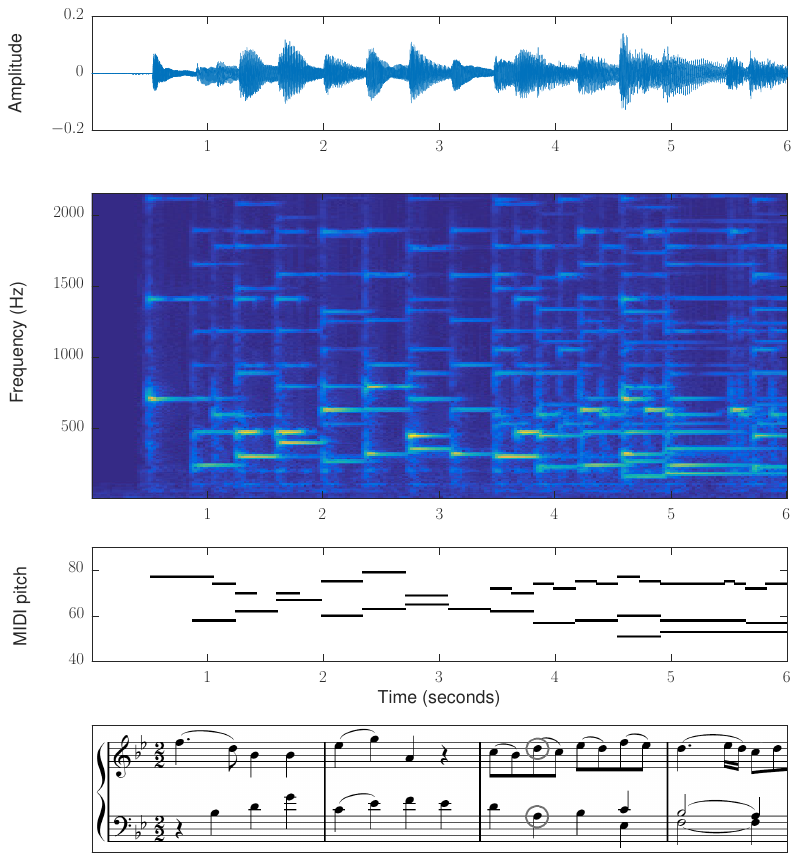
\includegraphics[width=12cm]{./statics/atm_data.png}
    \caption{نمایش‌های استفاده شده در یک سیستم \gls{ATM}.}
\end{figure}

در ادامه تلاش می‌شود به صورت مفصل‌تر به اهمیت و چالش‌های این مسئله پرداخته شود.

\subsection{کاربردها و تاثیرات}
یک سیستم \gls{atm} که بتواند به درستی کار کند، می‌تواند کاربردهای گسترده‌ای
همانند آموزش موسیقی، تولید موسیقی‌های جدید، جست‌وجو موسیقی و مطالعه موسیقی داشته
باشد. در نتیجه \gls{ATM} را می‌تواند تکنولوژی تاثیرگذار با منفعت اقتصادی و
اجتماعی بالا دانست.

\gls{atm} به صورت مستقیم با مسائل پردازش سیگنالی همچون جداسازی منبع‌های صوتی
مرتبط هست که هدف آن استخراج صوت تولیدی یک منبع خاص در مجموعه‌ای از اصوات ضبط شده
هست. نظیر با توجه به این که حل مسائل سطح بالایی همچنین تشخیص قطعات بازنوازی
شده و خوشه‌بندی قطعات موسیقی در حالت نوشتاری موسیقی بسیار ساده‌تر هست، می‌توان
یک سیستم \gls{ATM} را جزئی کلیدی برای حوزه \gls{mir} دانست. درنتیجه \gls{ATM}
حلقه اصلی ارتباط مسائل حوزه‌های پردازش سیگنال‌های موسیقی و پردازش نمادین موسیقی
هست.

باتوجه به تاثیر بالقوه یک سیستم \gls{atm}، علاوه بر تحقیقات آکادمیک، شرکت‌های
تجاری زیادی نیز به این مسئله علاقه‌مند شده‌اند. برای نمونه می‌توان از
نرم‌افزارهایی همچون Melodyne، AudioScore، ScoreCloud و Transcribe یاد کرد. هرچند
با توجه به تفاوت هدف نهایی این نرم‌افزارها مقایسه مستقیم عملکرد این نرم‌افزارها
با تحقیقات انجام شده، مقایسه‌ای عادلانه نخواهد بود.

\subsection{ارتباط و شباهت با سایر مسائل}
\gls{atm} ارتباطی بسیار نزدیک با سایر مسائل پردازش سیگنال دارد. یک سیستم
\gls{ATM} را می‌توان معادل یک سیستم \gls{asr} در حوزه پردازش گفتار دانست. شباهت
این دو سیستم از این جهت هست که هر دو سیستم تلاش می‌کنند یک سیگنال صوتی را تبدیل
به حالت نوشتاری اطلاعات کنند. همچنین مانند \gls{cocktail party problem} در
پردازش گفتار، موسیقی معمولا شامل چندین صدای همزمان هست. ولی برخلاف گفتار این
صداها به شدت به هم وابسته هستند. هر دوی سیستم‌های \gls{ATM}و \gls{ASR} می‌توانند
با یک \gls{language model} که در کنار \gls{acoustic model} استفاده می‌شود، دقت
را افزایش دهند. با توجه به این که موسیقی نیز مجموعه قواعد دستوری مخصوص به خود
دارد، ارتباطی مستقیم بین \gls{atm} و حوزه \gls{nlp} وجود دارد
\cite{boulanger2012modeling}.

در ادامه مسئله \gls{atm} با حوزه پردازش تصویر و بینایی ماشین نیز در ارتباط هست.
از آنجا که نمایش زمان-فرکانس مورد استفاده در این سیستم‌ها، یک نمایش دو بعدی هست،
می‌توان مسئله را به تشخیص نت‌ها در یک تصویر ورودی تقلیل داد. همچنین همانند اکثر
مسائل این حوزه که انسداد اجسام مورد مطالعه چالشی جدی هست، نت‌های موسیقی استفاده
شده در یک قطعه نیز، معمولا فضای یکسانی را در نمایش زمان-فرکانس مورد استفاده
اشغال می‌کنند.

\subsection{چالش‌ها}
در مقایسه با سایر مسائل حوزه پردازش سیگنال، چندین عامل باعث می‌شود تا مسئله
\gls{atm}، مسئله‌ای چالش‌برانگیز محسوب شود. موسیقی \gls{polyphonic} شامل چندین
منبع صوتی مختلف مانند ساز‌های مختلف و صدای خواننده هست. هر کدام از این منبع‌ها
قدرت صدا و \gls{timber} متفاوتی دارند. همچنین بعضی از این منابع صوتی می‌توانند
چندین نت را به صورت همزمان اجرا کنند. استنتاج ویژگی‌های موسیقیایی همانند
\gls{pitch} در حجمی از صداهای در هم تنیده، مسئله‌ای پیچیده محسوب می‌شود.

همچنین در یک قطعه موسیقی معمولا نت‌های استفاده با هم، دارای هارمونیک‌های یکسانی
نیز هستند. این همپوشانی هارمونیک‌ها مجددا باعث پیچیده‌تر شدن فرایند جداسازی
می‌شود. برای مثال یک آکورد دو ماژور را در نظر بگیرد. این آکورد شامل \gls{pitch}
های دو، می و سل می‌شود که فرکانس پایه آنها با هم نسبت ۴، ۵ و ۶ دارد. در نتیجه به
ترتیب ۴۶/۷, ۳۳/۳ و ۶۰ درصد هامونیک آن‌ها با هم همپوشانی دارد.

یکی دیگر از مشکلات، تبعیت زمان نت‌های موسیقیایی از ریتم و ساختار زمانی رایج در
موسیقی هست. برای مثال تلاش می‌شود که نت‌های مشابه زمان شروع و پایان یکسانی در
قطعات \gls{polyphonic} داشته باشند. این ارتباط زمانی نت‌ها با هم باعث می‌شود که
نتوان فرض مستقل بودن منابع صوتی مختلف را کرد که خود باعث پیچیده‌تر شدن جدا سازی
صوت‌های مختلف می‌شود.

مشکل دیگر این مسئله پیچیدگی انجام این فرایند حتی توسط موسیقی‌دانان با تجربه هست.
این پیچیدگی باعث می‌شود که گردآوری \gls{dataset} جامع فرایندی بسیار سخت و پر از
خطا باشد. حتی روش‌هایی مثل روش پیشنهاد شده در \cite{su2015escaping} نیاز به
نوازندگان خبره و پیش‌پردازش و پس‌پردازش سنگین دارد. همچنین قابل توجه هست که
\gls{sheet music} که قطعه از روی آن اجرا شده نیز نمی‌توان به عنوان یک برچسب قطعی
از داده استفاده شود. هر نوازنده با توجه به سلیقه خود ممکن است جاهایی از آهنگ را
تغییر دهد تا احساس مورد نظر را ایجاد کند. همچنین تشخیص این که هر نت متعلق به
کدام بازه زمانی سیگنال صوتی است هم به هیچ وجه مسئله‌ بدیهی محسوب نمی‌شود. در
نتیجه حتی در صورت وجود \gls{sheet music} قطعه، در بهترین حالت می‌توان آن را
برچسبی ضعیف برای سیگنال صوتی فرض کرد.

چالش‌های مطرح شده معمولا تمامشان در سیستم‌های کنونی کامل حل نمی‌شوند که منجر به
خطایی همچون نت‌های اضافه یا کم، اکتاوهای اشتباه، نت‌های ترکیب شده یا تجزیه شده و
زمان شروع و پایان اشتباه می‌شود.